\documentclass[11pt]{article}

\usepackage[margin=1.15in]{geometry}
\usepackage{amsmath}
\usepackage{amssymb}
\usepackage{graphicx}
\usepackage{xcolor}
\usepackage{booktabs}
\usepackage{tikz}
\usetikzlibrary{arrows.meta}

% One symbol per object, as in the project's other notes.
\newcommand{\kmax}{k_{\rm max}}
\newcommand{\hMpc}{\,h/{\rm Mpc}}
\newcommand{\kms}{\,{\rm km/s}}
\newcommand{\dcom}{$\Delta d_{\rm com} = 62$~Mpc}
% An underscore after which a long code name may break.
\newcommand{\us}{\_\allowbreak}

% Okabe-Ito colourblind-safe palette (the house palette).
\definecolor{OIorange}{HTML}{E69F00}
\definecolor{OIskyblue}{HTML}{56B4E9}
\definecolor{OIgreen}{HTML}{009E73}
\definecolor{OIyellow}{HTML}{F0E442}
\definecolor{OIblue}{HTML}{0072B2}
\definecolor{OIvermillion}{HTML}{D55E00}
\definecolor{OIpurple}{HTML}{CC79A7}

% A visible box for every number or figure that waits for a run.
\newcommand{\pending}[1]{%
  \begin{center}
  \fcolorbox{OIvermillion}{OIyellow!25}{\parbox{0.92\linewidth}{%
    \small\textbf{Pending --} #1}}
  \end{center}}

\title{Lensing magnification and the thin-bin cross spectra}
\date{November 2026}
\author{}

\emergencystretch=3em
% let the figures share a page with text
\renewcommand{\topfraction}{0.9}
\renewcommand{\bottomfraction}{0.8}
\renewcommand{\textfraction}{0.07}
\renewcommand{\floatpagefraction}{0.85}
\setcounter{topnumber}{3}
\setcounter{totalnumber}{4}

\begin{document}

\begin{center}
  {\LARGE Lensing magnification and the thin-bin cross spectra\par}
  \vspace{0.4em}
  {\large What magnification does to galaxy counts, what the forecast
    neglects by\\ setting its coefficient to zero, and the test that
    measures the cost\par}
  \vspace{0.6em}
  {\large November 2026\par}
\end{center}
\vspace{1em}

\section{Summary}
\label{sec:summary}

\paragraph{The setting.}
The project forecasts DESI galaxy clustering in thin redshift bins --
angular power spectra $C_\ell^{gg}$, computed without the Limber
approximation, joint with LSST~Y1 cosmic shear -- with Fisher
matrices: the forecast's error bars come from the derivatives of the
predicted data at one fiducial point.  That machinery is built step by
step in \texttt{notes/fisher\us machinery}; this note needs only its
vocabulary.  The data vector includes cross spectra between different
lens bins, and the companion note \texttt{notes/cross\us correlations}
shows that extending the measured pair list raises
${\rm FoM}(w_0, w_a)$ by up to $55$--$59\%$ on the three thinner
layouts.

\paragraph{The question.}
Light from a galaxy is deflected by the matter in front of it, and the
deflection changes how many galaxies a survey counts in each direction
-- an effect whose standard name, used once here and then replaced for
the reasons below, is \emph{magnification bias}.  In this project
``bias'' otherwise always means galaxy bias (the ratio of galaxy to
matter clustering), and a displacement of a recovered parameter is
always a ``shift'', never a bias.  So this note names the effect once,
and from here on speaks of the \emph{magnification coefficient} $C_i$
of lens bin $i$ (the number that multiplies the lensing convergence in
the observed counts, Section~\ref{sec:what}) and of the \emph{count
slope} $s$ (the property of the sample that sets $C_i$).  The forecast
currently sets $C_i = 0$ in every lens bin.  The question, raised by
the cross-correlation study: once more cross spectra are measured, does
the model need the magnification terms -- and does the answer change
between the paper's pair lists and the extended ones?

\paragraph{What is known without new runs.}
Three ingredients are already in hand.  (i)~\emph{The literature.}
DES~Y3 modelled exactly the term this project switches off, measured
its coefficients, and found that neglecting it shifts $S_8$ by up to
$0.85\sigma$ for its wider, deeper lens sample
\cite{ElvinPoole2022, KrauseY3}; Euclid's spectroscopic forecast finds
$0.2$--$0.7\sigma$ shifts from neglecting it even in a thin-bin
analysis without cross spectra, at higher redshift and larger
coefficients than DESI's \cite{EuclidSpectroMag}, and the neglected
term can also shift $n_s$ and the neutrino-mass sum
\cite{Cardona2016}; a dedicated
spectroscopic study finds the effect almost irrelevant for DESI's
samples because their coefficients are small, while flagging that the
coefficients need better modelling \cite{JelicCizmek2021}.
(ii)~\emph{The code audit.}  Cosmolike implements the DES~Y3 model --
one constant coefficient per lens bin times the bin's convergence --
correctly in its auto-spectrum paths, Limber and non-Limber; the one
hard restriction was that the gg cross-pair engine refused a nonzero
coefficient (\texttt{cosmo2D.c:13115}), keeping magnification off
exactly the spectra where it matters most
(Section~\ref{sec:cosmolike}).  (iii)~\emph{The pipeline numbers.}
The restriction of (ii) has since been lifted: the cross-pair engine
now carries the magnification rows, validated against the autos and
the existing vectors (Section~\ref{sec:guard}), and the shift test
ran at the final derivative tier on every layout and both pair lists
(Section~\ref{sec:shift}).  An earlier external Limber estimate,
recorded in Section~\ref{sec:estimate}, came out about ten times low
on the thin layouts and did not cover $\Delta z = 0.05$ and
$\Delta z = 0.2$; every conclusion below rests on the pipeline
numbers.

\paragraph{The answer in numbers.}
Every shift below is a what-if number -- if nature carries
magnification at the stated coefficients and the model leaves it out,
where does the fit land, in units of the forecast's own errors --
with no threshold line (Section~\ref{sec:shift},
Figure~\ref{fig:shift}).  At the measured coefficients (BGS $C = 2$,
LRG $C = 3$, ELG $0$), the thin-layout fits move by at most $0.07$ of
the error, on both pair lists: at those coefficients the thin-bin
forecasts, paper pairs or the extended ``pairmax'' pairs
(Section~\ref{sec:fiducial}), lose essentially nothing by
leaving magnification out.  The unmeasured ELG count slope dominates
the uncertainty: at the bracket corner $C_{\rm ELG} = +2$ the pairmax
lists reach $0.30$--$0.46$, and there the free nuisances
\emph{amplify} the shift rather than absorb it -- the magnification
excess on the added pairs reads as a change of the per-group
linear-bias level and slope, the same freedom that produces the
pairmax FoM gain, so the gain and the magnification sensitivity
travel together.  At $C_{\rm ELG} = -2$ the paper lists themselves
reach $0.2$--$0.3$.  The wide $\Delta z = 0.2$ layout is
magnification dominated -- its measured adjacent cross spectra change
by up to $25$ times their magnification-free size -- and moves
$0.19$ even at the measured
coefficients, with $A_s$ shifting by about $1\sigma$ at
$C_{\rm ELG} = +2$.  Measuring the ELG count slope
(Section~\ref{sec:measure}) is therefore the study's single most
valuable next step.

\section{Fiducial model and parameter values}
\label{sec:fiducial}

Every number of this note is computed at the fiducial below, the
evaluate point -- the parameter values at which the data vectors and
derivatives are evaluated -- of the paper configurations
\texttt{EXAMPLE\us EVALUATE1}--\texttt{4.yaml}, frozen here so the
note does not depend on files that may change.

\paragraph{Cosmology.}
Flat $w_0 w_a$CDM: $10^9 A_s = 2.1$ ($A_s$ the amplitude of the
primordial curvature power spectrum), $n_s = 0.96605$,
$H_0 = 67.32$~km/s/Mpc, $\Omega_b = 0.04$, $\Omega_m = 0.3$ (neutrinos
included), $w_0 = -1$ and $w_a = 0$; the neutrino mass sum is
$0.06$~eV and the optical depth $\tau = 0.0697$; derived
$\sigma_8 = 0.8278$.  The Fisher matrices vary $10^9 A_s$, $n_s$,
$H_0$, $\Omega_b$, $\Omega_m$, $w_0$ and $w_a$ with flat priors.

\paragraph{Layouts, bands and pair lists.}
Four lens-bin layouts: \dcom{} ($76$ bins), $\Delta z = 0.02$ ($90$),
$\Delta z = 0.05$ ($36$) and $\Delta z = 0.2$ ($10$); every spectrum
is measured in $53$ band powers of width $\Delta\ell = 10$ over
$15 \le \ell \le 544$.  The \emph{paper pair lists} keep the cross
pairs whose blurred redshift distributions overlap by at least
$10^{-6}$ at the fiducial velocity dispersions
(\texttt{data/<stem>\us pairs.txt}): $107$, $133$, $52$ and $13$
pairs on the four layouts.  The \emph{pairmax lists} of the pair-axes
study ($378$, $370$, $178$ and $32$ pairs) add deeper pairs, with a
reach that differs by layout.  Writing $g$ for the distance between
the two bins' raw redshift ranges in bin widths -- the convention of
\texttt{notes/cross\us correlations}, in which an adjacent pair has
$g = 0$ and $C_\ell^{i,i+2}$ has $g = 1$ -- the pairmax lists keep
$g \le 3$ on \dcom{} and $\Delta z = 0.05$, $g \le 2$ on
$\Delta z = 0.2$, and on $\Delta z = 0.02$ the pairs with $g \le 2$
plus those of the $\sigma_v = 450$, $600$, $750$, $900$ and
$1200\kms$ overlap lists (the overlap criterion rerun with every
group's dispersion set to that one value).  How far apart the listed pairs are
\emph{in distance} varies strongly by layout
(Section~\ref{sec:handworked}, Table~\ref{tab:efficiency}): the thin
layouts' lists are radially local, the $\Delta z = 0.2$ list is not.
The forecast sky is
$12{,}300$~deg$^2$; the covariance is Gaussian, built at
$14{,}000$~deg$^2$ with its inverse rescaled by $12{,}300/14{,}000$.

\paragraph{Galaxy bias.}
The group amplitudes are $B_g = 1.34$ (BGS), $1.7$ (LRG1--LRG3) and
$0.84$ (ELG1, ELG2); at the fiducial every tilt and residual is zero,
so bin $i$ has linear bias $b_{1,i} = B_g/D(\bar{z}_i)$, with the
growth factor $D$ ($D = 1$ today) read off the linear power spectrum
at $k = 0.005~{\rm Mpc}^{-1}$ and $\bar{z}_i$ the bin's mean redshift.
The one-loop terms are those of the fiducial model: quadratic and
tidal biases on their calibrations, $\alpha_2 = 0$ in every bin, the
stochastic amplitudes zero, the pessimistic linear-bias prior, and
every velocity-dispersion prior width six times its base width
(\texttt{notes/bias\us model\us summary}).

\paragraph{Velocity dispersions.}
Seven dispersion groups with fiducials $371$, $358$, $357$, $348$,
$343$, $304$ and $289\kms$ (BGS split at $\bar z = 0.255$); each thin
bin's redshift distribution is convolved with the group's Gaussian
blur before any kernel is built.

\paragraph{Scale cuts.}
The non-Limber ultraviolet-fraction scale cut \cite{Saraivanov2026}:
bin $i$ is cut at $\kmax/D(\bar z_i)$, and a band is kept while less
than $5\%$ of it comes from the power spectrum above that cut,
intersected with the shipped mask ($k = 0.1185~{\rm Mpc}^{-1}$, about
$0.176\hMpc$, in every bin).  As everywhere in this project, a quoted
$\kmax$ is the value at $z = 0$.

\paragraph{Magnification coefficients.}
The fiducial coefficients adopted for the tests, with the measured
count slopes behind them (defined and derived in
Section~\ref{sec:what}; sources in Table~\ref{tab:coeff}): BGS
$C = +2.0$, LRG $C = +3.0$, ELG bracketed in $C \in [-2, +2]$ with $0$
as the central value.  One constant per sample group, assigned to
every bin of the group.

\section{What lensing magnification is}
\label{sec:what}

This section builds the effect from the ground up.  Nothing in it is
specific to this project; everything downstream depends on it.

\subsection{The magnifying-glass picture}
\label{sec:glass}

Light travels to us through a lumpy universe.  Where the line of
sight passes more matter than average, the extra gravity bends the
rays toward the mass, exactly as a glass lens bends rays toward its
axis.  A patch of sky behind an overdense foreground therefore
behaves as if seen through a weak magnifying glass: everything in the
patch looks slightly \emph{larger} and, because the bending conserves
surface brightness (photons are neither created nor destroyed, only
redirected), slightly \emph{brighter}.  Behind an underdense
foreground the same logic runs in reverse: a weak reducing glass.
The magnification varies from direction to direction, tracing the
foreground matter -- and that is the whole effect.  Everything below
is bookkeeping of what a magnifying glass does to galaxy counts.

\subsection{Convergence, shear, and $\mu \simeq 1 + 2\kappa$}
\label{sec:kappa}

Two numbers describe the distortion of a small patch of sky.  The
\emph{convergence} $\kappa$ is the isotropic part: positive $\kappa$
enlarges images in all directions equally.  The \emph{shear} $\gamma$
is the anisotropic part: it stretches images along one axis and
squeezes them along the other, turning circles into ellipses, and is
the quantity cosmic-shear surveys measure.  Formally, the mapping
from true to observed positions has the Jacobian matrix
\begin{equation}
  A =
  \begin{pmatrix}
    1 - \kappa - \gamma_1 & -\gamma_2 \\
    -\gamma_2 & 1 - \kappa + \gamma_1
  \end{pmatrix},
\end{equation}
whose determinant is the ratio of true to observed solid angle.  The
\emph{magnification} $\mu$ is the ratio of observed to true solid
angle, the inverse determinant:
\begin{equation}
  \mu \;=\; \frac{1}{\det A}
       \;=\; \frac{1}{(1-\kappa)^2 - |\gamma|^2}
       \;\simeq\; 1 + 2\kappa ,
  \label{eq:mu}
\end{equation}
where the last step expands to first order in $\kappa$ and $\gamma$,
the weak-lensing limit ($\kappa, |\gamma| \ll 1$): the shear enters
$\mu$ only at second order, so to first order magnification is set by
the convergence alone.  For scale: along a typical line of sight to
$z \sim 1$, $\kappa$ is of order $10^{-2}$ at most, so
$\mu - 1 \lesssim 2\%$.

Physically, $\kappa$ in a given direction is the matter overdensity
along the line of sight, weighted by how efficiently each distance
lenses (Section~\ref{sec:efficiency} derives the weight):
\begin{equation}
  \kappa_j(\hat{\mathbf n})
  = \int_0^{\chi_j} d\chi\, W_{{\rm mag},j}(\chi)\,
    \delta_m(\chi\hat{\mathbf n}, \chi),
  \label{eq:kappadef}
\end{equation}
with $\delta_m$ the matter density contrast, $\chi$ the comoving
distance, and $W_{{\rm mag},j}$ the lensing-efficiency kernel of the
galaxies of bin $j$.  The subscript $j$ matters: each lens bin has
its own convergence, sourced by the matter in front of \emph{its}
galaxies.

\subsection{The two competing effects on counts}
\label{sec:twoeffects}

A survey counts galaxies per unit solid angle above a flux limit.
Magnification changes both the solid angle and the fluxes
(Figure~\ref{fig:twoeffects}):

\begin{enumerate}
\item \textbf{Area dilution.}  A patch of true solid angle
  $\Delta\Omega$ is observed with solid angle $\mu\,\Delta\Omega$:
  the same galaxies are spread over more sky, so the observed number
  density \emph{drops} by the factor $\mu$.  With
  Eq.~\eqref{eq:mu}, that is a contribution $-2\kappa$ to the
  observed density contrast.
\item \textbf{Flux brightening.}  Each galaxy's image area grows by
  $\mu$ while its surface brightness (flux per unit image area) is
  conserved, so its total flux grows by $\mu$.  Galaxies that sat
  just below the survey's flux limit are lifted \emph{into} the
  sample, so the counts \emph{rise} -- by an amount set by how many
  galaxies sit just below the limit, i.e.\ by the steepness of the
  counts at the limit.
\end{enumerate}

Which effect wins depends on the sample, through one number, defined
next.

\begin{figure}[tbp]
  \centering
  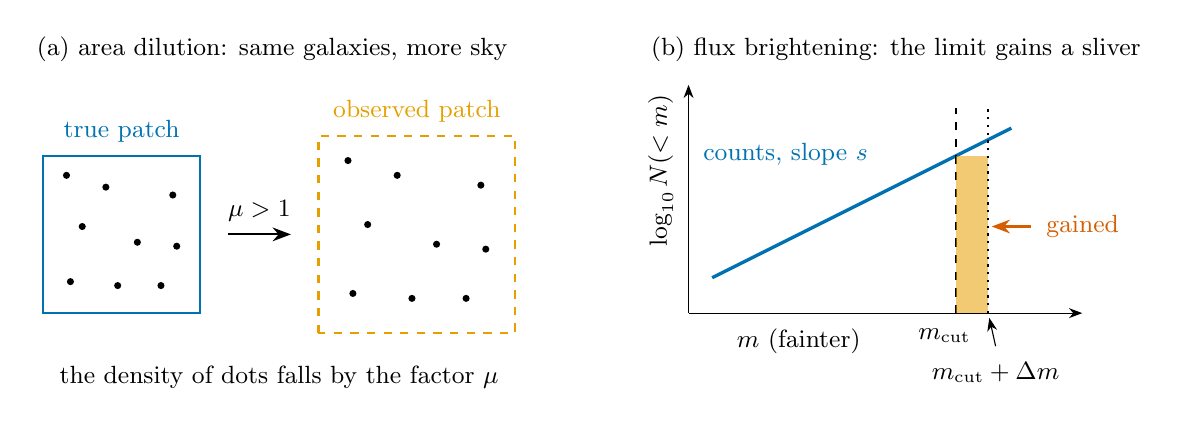
\begin{tikzpicture}[x=1cm, y=1cm, font=\small, >=Stealth]
    % ---- Panel (a): area dilution -------------------------------
    \node[anchor=west] at (-0.2, 3.35) {(a) area dilution: same galaxies, more sky};
    % true patch
    \draw[OIblue, thick] (0, 0) rectangle (2.0, 2.0);
    \node[OIblue, anchor=south] at (1.0, 2.05) {true patch};
    \foreach \x/\y in {0.35/0.4, 0.8/1.6, 1.2/0.9, 1.65/1.5, 0.5/1.1,
                       1.5/0.35, 0.95/0.35, 1.7/0.85, 0.3/1.75}
      \fill[black] (\x, \y) circle (0.045);
    % arrow
    \draw[->, thick] (2.35, 1.0) -- (3.15, 1.0)
      node[midway, above=1pt] {$\mu > 1$};
    % observed patch (stretched by factor 1.25)
    \draw[OIorange, thick, dashed] (3.5, -0.25) rectangle (6.0, 2.25);
    \node[OIorange, anchor=south] at (4.75, 2.3) {observed patch};
    \foreach \x/\y in {0.35/0.4, 0.8/1.6, 1.2/0.9, 1.65/1.5, 0.5/1.1,
                       1.5/0.35, 0.95/0.35, 1.7/0.85, 0.3/1.75}
      \fill[black] ({3.5 + 1.25*\x}, {-0.25 + 1.25*\y}) circle (0.045);
    \node[anchor=north, align=center] at (3.0, -0.55)
      {the density of dots falls by the factor $\mu$};
    % ---- Panel (b): flux brightening ----------------------------
    \begin{scope}[shift={(8.2, 0)}]
      \node[anchor=west] at (-0.6, 3.35) {(b) flux brightening: the limit gains a sliver};
      % axes
      \draw[->] (0, 0) -- (5.0, 0);
      \node[anchor=north] at (1.4, -0.08) {$m$ (fainter)};
      \draw[->] (0, 0) -- (0, 2.9) node[rotate=90, anchor=south east, yshift=2pt] {$\log_{10} N(<m)$};
      % counts line, slope s
      \draw[OIblue, very thick] (0.3, 0.45) -- (4.1, 2.35);
      \node[OIblue, anchor=south east, align=right] at (2.4, 1.75) {counts, slope $s$};
      % flux limit
      \draw[black, dashed, thick] (3.4, 0) -- (3.4, 2.6);
      \node[anchor=north] at (3.25, -0.08) {$m_{\rm cut}$};
      % gained sliver
      \fill[OIorange, opacity=0.55] (3.4, 0) rectangle (3.8, 2.0);
      \draw[black, dotted, thick] (3.8, 0) -- (3.8, 2.6);
      \node[anchor=north] at (3.9, -0.5) {$m_{\rm cut} + \Delta m$};
      \draw[->, thin] (3.9, -0.42) -- (3.82, -0.06);
      \draw[->, OIvermillion, thick] (4.35, 1.1) -- (3.85, 1.1);
      \node[OIvermillion, anchor=west, align=left, font=\small]
        at (4.42, 1.1) {gained};
    \end{scope}
  \end{tikzpicture}
  \caption{The two competing effects of a magnification $\mu > 1$ on
    galaxy counts.  (a)~Area dilution: the observed patch (dashed
    orange) covers $\mu$ times the solid angle of the true patch
    (solid blue) and holds the same galaxies, so the number density
    falls by $\mu$.  (b)~Flux brightening: each galaxy brightens by
    $\mu$, which shifts the effective magnitude limit faintward by
    $\Delta m = 2.5\log_{10}\mu$; the sample gains the galaxies in
    the shaded sliver, a fraction set by the count slope $s$ (the
    slope of the blue line at the cut).  The net effect is the
    difference of the two.}
  \label{fig:twoeffects}
\end{figure}

\subsection{The count slope $s$}
\label{sec:slope}

Let $N(<m)$ be the cumulative number of sample galaxies per unit
solid angle brighter than apparent magnitude $m$ (recall that larger
$m$ means fainter: $m = -2.5\log_{10} F + {\rm const}$, with $F$ the
flux).  The \emph{count slope} at the sample's magnitude limit
$m_{\rm cut}$ is
\begin{equation}
  s \;\equiv\; \frac{d\log_{10} N(<m)}{dm}\bigg|_{m_{\rm cut}} .
  \label{eq:s}
\end{equation}
It answers: if the survey could see $0.1$~magnitude deeper, by what
fraction would the sample grow?  (By $10^{0.1 s} - 1 \approx
0.23\,s$.)  A steep luminosity function near the cut gives large $s$;
a sample whose counts have flattened near the cut (a bright,
nearly complete sample) gives small $s$.  An equivalent convention
uses the counts as a function of flux, $n(>F) \propto F^{-\alpha}$;
since $F \propto 10^{-0.4 m}$, the two slopes are related by
\begin{equation}
  \alpha = 2.5\, s .
  \label{eq:alpha}
\end{equation}

\subsection{The derivation of $\delta_\mu = (5s - 2)\,\kappa$, step by step}
\label{sec:derivation}

Work in one direction $\hat{\mathbf n}$ with magnification $\mu$, and
compare the observed number density $n_{\rm obs}$ (per observed solid
angle, above the observed flux limit $F_{\rm cut}$) with the density
$n_0$ that would be observed with no lensing.

\paragraph{Step 1: what magnification does to the inputs.}
Fluxes: every galaxy's observed flux is $\mu$ times its unlensed
flux, so a galaxy passes the cut if its unlensed flux exceeds
$F_{\rm cut}/\mu$.  Solid angle: a patch holding the galaxies has
observed solid angle $\mu$ times its true solid angle.

\paragraph{Step 2: the observed density.}
Therefore
\begin{equation}
  n_{\rm obs}(>F_{\rm cut})
  = \frac{1}{\mu}\; n_0\!\left(> \frac{F_{\rm cut}}{\mu}\right):
\end{equation}
the $1/\mu$ in front is the area dilution; the deeper effective limit
$F_{\rm cut}/\mu$ is the brightening.

\paragraph{Step 3: expand the counts at the limit.}
Near the cut the counts behave as a power law,
$n_0(>F) \propto F^{-\alpha}$ with $\alpha$ the flux slope of
Eq.~\eqref{eq:alpha}.  Then
\begin{equation}
  n_0\!\left(> \frac{F_{\rm cut}}{\mu}\right)
  = \mu^{\alpha}\, n_0(>F_{\rm cut}),
  \qquad\text{so}\qquad
  n_{\rm obs} = \mu^{\alpha - 1}\, n_0 .
  \label{eq:mualpha}
\end{equation}

\paragraph{Step 4: linearize.}
With $\mu \simeq 1 + 2\kappa$ from Eq.~\eqref{eq:mu} and
$\kappa \ll 1$,
\begin{equation}
  \frac{n_{\rm obs} - n_0}{n_0}
  \;\equiv\; \delta_\mu
  \;=\; (\alpha - 1)\, 2\kappa
  \;=\; (5s - 2)\,\kappa .
  \label{eq:deltamu}
\end{equation}
The same arithmetic in magnitude language, as a check: the
brightening shifts every magnitude by
$\Delta m = -2.5\log_{10}\mu \simeq -(5/\ln 10)\,\kappa$, so the
sample gains a fraction
$\ln 10 \cdot s \cdot |\Delta m| = 5 s\,\kappa$ (the sliver of
Figure~\ref{fig:twoeffects}b), while the dilution removes $2\kappa$;
the net is $(5s - 2)\,\kappa$.

\paragraph{The worked toy: $s = 0.4$ cancels.}
Take $\kappa = 0.01$, so $\mu = 1.02$: the patch grows by $2\%$ and
every galaxy brightens by $2\%$ ($\Delta m \simeq -0.0215$~mag).  For
a sample with $s = 1$ (the DESI LRGs, Table~\ref{tab:coeff}), the
brightening pulls in $5 s \kappa = 5\%$ more galaxies while the
dilution costs $2\%$: the counts rise by $3\%$, i.e.\ $C = +3$.  For
a sample with $s = 0.4$ the gain is $5 \times 0.4 \times 0.01 = 2\%$,
exactly the dilution: the counts do not change at all, however strong
the lensing.  For a bright, flat-counts sample with $s = 0.2$ the
gain is only $1\%$ and the counts \emph{drop} by $1\%$: behind an
overdensity such a sample looks emptier, $C = -1$.

\subsection{The conventions map}
\label{sec:conventions}

One effect, several notations in the literature and the code.  All of
the following are the same number:
\begin{equation}
  C \;=\; 5s - 2 \;=\; 2(\alpha - 1)
  \;=\; \texttt{b\us mag}\ \text{(cosmolike)} .
  \label{eq:conventions}
\end{equation}
DES~Y3 \cite{KrauseY3, ElvinPoole2022} writes
$\delta_\mu = C\,\kappa$ and splits $C = C_{\rm sample} + C_{\rm
area}$ with $C_{\rm area} = -2$ and $C_{\rm sample}$ the measured
response of the selection ($C_{\rm sample} = 5s$ for a pure magnitude
cut; their general definition also covers size selection, adding a
size-slope term $\partial\ln n/\partial\ln r$ at the cut
\cite{KrauseY3}).  Cosmolike's per-bin nuisance parameter
\texttt{b\us mag} multiplies the convergence kernel directly, so it
is the \emph{total} coefficient $C$, area term included -- any wiring
of measured slopes must set $\texttt{b\us mag} = 5s - 2$, never $s$.
In this note the symbol is $C_i$, the magnification coefficient of
lens bin $i$.

\subsection{How $s$ is measured for a real selection}
\label{sec:measure}

For a pure magnitude-limited sample, $s$ can be read off the
luminosity function.  Real selections are not pure magnitude cuts --
they combine colours, total magnitudes, fibre magnitudes and sizes --
and then the only reliable method is the \emph{finite difference}: take
the target catalog, shift every magnitude by a small
$\delta m = \pm 0.01$ (the response of each quantity to
magnification applied individually), re-run the full selection, and
difference the counts \cite{ElvinPoole2022, Zhou2023, Wenzl2023}.  Two
subtleties move the answer by tens of percent:

\begin{itemize}
\item \textbf{Fibre magnitudes respond less than total magnitudes.}
  A fibre magnitude measures the flux inside a fixed aperture.  A
  magnified galaxy is brighter \emph{and larger}, so a smaller
  fraction of its flux falls inside the aperture: the fibre flux
  rises by less than $\mu$.  A selection with fibre-magnitude cuts
  (DESI's LRG and ELG selections have them) therefore responds less
  than the total-magnitude arithmetic suggests.  Ignoring this
  overestimates the DESI LRG slope by ${\sim}13\%$ for the full
  sample and ${\sim}30\%$ in its faintest bin \cite{Zhou2023} -- and
  the signal scales with $s - 0.4$, which amplifies the error
  further.
\item \textbf{Size cuts respond with the opposite sign.}  A cut that
  rejects large images (star--galaxy separation does) loses galaxies
  when magnification enlarges them, partially cancelling the flux
  gain.  DES~Y3 found its image-simulation estimates (which carry
  the size response) systematically below its flux-only estimates for
  this reason \cite{ElvinPoole2022}.
\end{itemize}

Within one sample the slope also drifts with redshift -- by up to a
factor of three across the BOSS CMASS sample \cite{Wenzl2023} -- which
is why a per-bin coefficient (Section~\ref{sec:cosmolike}) is the
right level of modelling for thin bins.

\subsection{The measured DESI values}
\label{sec:desivalues}

Table~\ref{tab:coeff} collects the measured count slopes for the DESI
samples and the coefficients adopted by this study.  The LRG and BGS
slopes are finite-difference measurements on the DESI target
catalogs; no equivalent measurement exists for the ELGs, whose
published values are luminosity-function models only
\cite{JelicCizmek2021}, so the study brackets $C_{\rm ELG}$ and
treats the measurement as an open item
(Appendix~\ref{sec:open}).

\begin{table}[tbp]
  \centering
  \small
  \begin{tabular}{lccl}
    \toprule
    sample & count slope $s$ & adopted $C = 5s - 2$ & source \\
    \midrule
    BGS & $0.81,\ 0.80$ (two bins, $z_{\rm eff} = 0.21,\ 0.35$)
        & $+2.0$ & finite diff.\ \cite{Sailer2025} \\
    LRG & $0.97$--$1.04$ per bin; $1.008 \pm 0.007$ full
        & $+3.0$ & finite diff.\ \cite{Zhou2023} \\
        & $0.999 \pm 0.015$ (DECaLS, DESI-like)
        &        & also \cite{KitanidisWhite2020} \\
    ELG & no measurement; models only
        & $0$, bracket $[-2, +2]$ & \cite{JelicCizmek2021} \\
    \bottomrule
  \end{tabular}
  \caption{Measured count slopes of the DESI samples and the
    magnification coefficients this study adopts (one constant per
    sample group).  The LRG and BGS slopes include the fibre-flux and
    photometric-redshift responses (Section~\ref{sec:measure}).  The
    ELG bracket spans the plausible range of a faint,
    colour-selected sample; the finite-difference measurement on the
    DESI ELG selection is an open item.}
  \label{tab:coeff}
\end{table}

\pending{T0 (optional): finite-difference count slopes per thin bin
for BGS, LRG and ELG from the DESI target selections, with the
fibre-magnitude response; one figure $s(z)$ per sample.  Until it
runs, Table~\ref{tab:coeff} holds group constants and the ELG
bracket.}

\section{Why cross spectra see it most}
\label{sec:cross}

\subsection{The lensing efficiency, step by step}
\label{sec:efficiency}

How strongly does matter at distance $\chi$ lens a source at distance
$\chi_s$?  Three factors build the answer.

\paragraph{Step 1: the deflection.}
A lump of matter at $\chi$ bends a passing ray by an angle
proportional to the lump's mass -- more precisely, to the transverse
gradient of its gravitational potential.  Through Poisson's equation
that gradient traces $\Omega_m\,\delta_m/a$, with $a$ the scale
factor at the lens (the $1/a$ because the potential of a fixed
comoving overdensity grows as the universe expands around it).

\paragraph{Step 2: the geometry.}
A fixed deflection at the lens displaces the \emph{apparent} source
position by an angle proportional to $(\chi_s - \chi)/\chi_s$: a
deflection right at the source ($\chi = \chi_s$) moves its image not
at all, a deflection halfway moves it most effectively relative to
the lever arms.  One more factor $\chi$ converts the angular scale of
the lensing mass to a transverse physical scale.  The product
$\chi\,(\chi_s - \chi)/\chi_s$ is the famous lensing-efficiency
triangle: zero at the observer, zero at the source, broad maximum
halfway in between.

\paragraph{Step 3: average over the bin.}
The galaxies of lens bin $j$ are distributed in distance as the bin's
(blurred) $n_j(\chi)$, so the kernel of Eq.~\eqref{eq:kappadef}
averages the triangle over the bin:
\begin{equation}
  W_{{\rm mag},j}(\chi)
  = \frac{3\Omega_m H_0^2}{2 c^2}\,
    \frac{\chi}{a(\chi)}
    \int_\chi^{\infty} d\chi'\; n_j(\chi')\,
    \frac{\chi' - \chi}{\chi'} .
  \label{eq:wmag}
\end{equation}
For a thin bin at $\chi_j$ the inner integral is simply
$(\chi_j - \chi)/\chi_j$.  The kernel is \emph{broad}: it extends
from the observer to the bin, whatever the bin's width.  That
breadth, against the thinness of the density kernels, drives
everything in this note (Figure~\ref{fig:geometry}).

\begin{figure}[tbp]
  \centering
  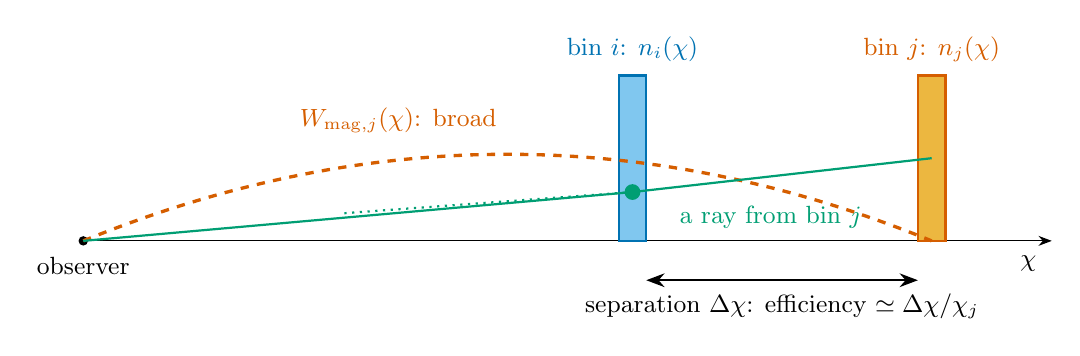
\begin{tikzpicture}[x=1cm, y=1cm, font=\small, >=Stealth]
    % axis
    \draw[->] (0, 0) -- (12.3, 0) node[below left=2pt] {$\chi$};
    \node[anchor=north] at (0, -0.08) {observer};
    \fill[black] (0, 0) circle (0.06);
    % bin i (density kernel, thin, tall)
    \fill[OIskyblue, opacity=0.75] (6.8, 0) rectangle (7.15, 2.1);
    \draw[OIblue, thick] (6.8, 0) rectangle (7.15, 2.1);
    \node[OIblue, anchor=south] at (6.975, 2.15) {bin $i$: $n_i(\chi)$};
    % bin j (density kernel, thin, tall)
    \fill[OIorange, opacity=0.75] (10.6, 0) rectangle (10.95, 2.1);
    \draw[OIvermillion, thick] (10.6, 0) rectangle (10.95, 2.1);
    \node[OIvermillion, anchor=south] at (10.775, 2.15) {bin $j$: $n_j(\chi)$};
    % magnification kernel of j: parabola chi(chi_j - chi)/chi_j, peak at chi_j/2
    % chi_j ~ 10.775; peak height scaled to 1.1
    \draw[OIvermillion, very thick, dashed, domain=0:10.775, samples=60]
      plot (\x, {1.1*4*\x*(10.775-\x)/(10.775*10.775)});
    \node[OIvermillion, anchor=south] at (4.0, 1.25)
      {$W_{{\rm mag},j}(\chi)$: broad};
    % light ray from a galaxy in bin j, bent at a lens inside bin i
    \fill[OIgreen] (6.975, 0.62) circle (0.10);
    \draw[OIgreen, thick] (10.775, 1.05) -- (6.975, 0.62) -- (0, 0.0);
    \draw[OIgreen, thick, dotted] (6.975, 0.62) -- (3.3, 0.35);
    \node[OIgreen, anchor=west, align=left, font=\small] at (7.45, 0.30)
      {a ray from bin $j$};
    % efficiency annotation between bins
    \draw[<->, thick] (7.15, -0.5) -- (10.6, -0.5);
    \node[anchor=north] at (8.875, -0.55)
      {separation $\Delta\chi$: efficiency $\simeq \Delta\chi/\chi_j$};
  \end{tikzpicture}
  \caption{The geometry of lens-bin magnification.  The density
    kernels of two thin bins (solid boxes) are narrow and disjoint,
    so their density cross spectrum is tiny.  The magnification
    kernel of the farther bin (dashed curve,
    Eq.~\eqref{eq:wmag}) is broad: it covers the whole foreground,
    bin $i$ included, so the matter that bin $i$'s galaxies trace
    also magnifies bin $j$'s counts (green ray).  At bin $i$'s
    location the kernel's height is the lensing efficiency
    $\simeq \Delta\chi/\chi_j$ times $(1+z_i)\,\chi_i$
    (Eq.~\eqref{eq:height}): small for close pairs, large for far
    ones.}
  \label{fig:geometry}
\end{figure}

\subsection{Hand-worked efficiencies and kernel heights}
\label{sec:handworked}

Two numbers describe how strongly a pair $(i, j)$, $\chi_i < \chi_j$,
couples density to magnification.  The first is the \emph{efficiency}
of Eq.~\eqref{eq:wmag} at the nearer bin,
$(\chi_j - \chi_i)/\chi_j = \Delta\chi/\chi_j$.  The second -- the one
that actually sets the cross term -- is the \emph{kernel height},
the full kernel at bin $i$:
\begin{equation}
  W_{{\rm mag},j}(\chi_i)
  = \frac{3\Omega_m H_0^2}{2c^2}\,(1 + z_i)\,\chi_i\,
    \frac{\Delta\chi}{\chi_j}
  \;\equiv\; \frac{3\Omega_m H_0^2}{2c^2}\; h_{ij},
  \qquad
  h_{ij} = (1 + z_i)\,\chi_i\,\frac{\Delta\chi}{\chi_j} .
  \label{eq:height}
\end{equation}
For radially close pairs $\chi_i \approx \chi_j$, so
$h_{ij} \approx (1 + z_i)\,\Delta\chi$: pairs with the same radial
separation have nearly the same kernel height wherever they sit.  A
low-redshift pair can therefore carry a large \emph{efficiency}
($\chi_j$ is small) and still a modest kernel: the small
$(1 + z_i)\,\chi_i$ gives back what the efficiency gained.

Worked cases, by hand, quoting $h_{ij}$ in Mpc (the prefactor is
common to all).  Pair depth uses the $g$ convention of
Section~\ref{sec:fiducial} (adjacent $= g = 0$).  The thin
$\Delta z = 0.02$ bins are $\approx 55$~Mpc wide; near the ELG range
$\chi \approx 3200$~Mpc (the distance the cross-correlations note's
toy uses at $z = 0.93$):

\begin{itemize}
\item \textbf{Adjacent pair, $g = 0$ (the paper lists):} centres one
  bin width apart, $\Delta\chi \approx 55$~Mpc:
  efficiency $\approx 55/3255 \approx 0.017$,
  $h \approx 1.92 \times 3200 \times 0.017 \approx 100$~Mpc.
\item \textbf{Added pair, $g = 2$ (the pairmax lists):} centres three
  widths apart, $\Delta\chi \approx 165$~Mpc:
  efficiency $\approx 0.049$, $h \approx 300$~Mpc.  The deepest
  thin-layout additions, $g = 3$ (centres four widths apart,
  $\Delta\chi \approx 220$~Mpc), reach efficiency $\approx 0.064$ and
  $h \approx 390$~Mpc.
\item \textbf{A far pair (in no current list):} BGS at $z = 0.3$
  ($\chi \approx 1250$~Mpc) against an ELG bin at $z = 0.92$:
  efficiency $\approx (3200 - 1250)/3200 \approx 0.61$, ten times the
  $g = 3$ value -- but
  $h \approx 1.30 \times 1250 \times 0.61 \approx 990$~Mpc, only
  $2.5$--$3$ times the added pairs' heights: the small
  $(1+z_i)\,\chi_i$ at low redshift gives back most of the
  efficiency gain.  The measured totals of
  Table~\ref{tab:dchi2} fold the coefficients, biases and band
  errors on top of these heights.
\end{itemize}

The same offset defuses the largest paper-list efficiencies of the
thin layouts, which sit at their lowest-redshift BGS adjacent pairs:
on $\Delta z = 0.02$ the pair $\bar z = 0.110 \times 0.130$ has
$\Delta\chi/\chi_j \approx 0.15$ -- the largest on that paper list --
but $h \approx 1.11 \times 480 \times 0.15 \approx 80$~Mpc, below the
ELG adjacent pair's $\approx 100$~Mpc.

Table~\ref{tab:efficiency} gives the efficiencies of every listed
pair, evaluated at the bin mean redshifts.  The layouts differ in
kind.  The thin layouts' paper lists are radially local (median
efficiencies $1.5$--$4\%$, maxima at the defused low-$z$ BGS pairs),
and their pairmax lists reach $0.34$--$0.59$ only at single deep
pairs.  On $\Delta z = 0.2$ \emph{every} pair is far apart in this
sense: its adjacent BGS pair ($\bar z = 0.203 \times 0.345$) has
efficiency $0.39$ and $h \approx 1.20 \times 860 \times 0.39 \approx
400$~Mpc -- the kernel height of a thin-layout $g = 3$ pair, on a
\emph{measured} paper pair -- and even its cross-sample
LRG2$\,\times\,$ELG1 pair ($\bar z = 0.706 \times 0.906$) has
efficiency $0.18$, where the thin layouts' cross-sample pairs sit at
essentially the same redshift with $\Delta\chi \approx 0$.  The
$\Delta z = 0.2$ layout is the most DES-like -- wide bins, large
separations, and by the mode counting of Section~\ref{sec:modes} the
largest relative weight of magnification per spectrum; the DES lens
bins that made magnification a headline systematic span the survey
depth with efficiencies of order one half \cite{ElvinPoole2022}.
Sections~\ref{sec:estimate} and~\ref{sec:shift} confirm what this
geometry predicts: the wide layout's cross spectra are magnification
dominated, and its shifts are the largest of the four layouts.

\begin{table}[tbp]
  \centering
  \begin{tabular}{lcc}
    \toprule
    layout & paper list: median / max & pairmax list: median / max \\
    \midrule
    \dcom{}           & $0.020$ / $0.120$ & $0.056$ / $0.351$ \\
    $\Delta z = 0.02$ & $0.015$ / $0.149$ & $0.032$ / $0.342$ \\
    $\Delta z = 0.05$ & $0.038$ / $0.271$ & $0.094$ / $0.589$ \\
    $\Delta z = 0.2$  & $0.132$ / $0.390$ & $0.250$ / $0.672$ \\
    \bottomrule
  \end{tabular}
  \caption{The lensing efficiency $\Delta\chi/\chi_j$ of every pair
    of the paper and pairmax lists, evaluated at the bin mean
    redshifts for flat $\Lambda$CDM with $\Omega_m = 0.3$ and
    $h = 0.6732$: the median and the maximum per list.  The thin
    layouts' paper lists are radially local; the $\Delta z = 0.2$
    lists are not.  The efficiency alone overstates the low-redshift
    pairs: the kernel height of Eq.~\eqref{eq:height} carries the
    extra factor $(1 + z_i)\,\chi_i$, which defuses them
    (Section~\ref{sec:handworked}).}
  \label{tab:efficiency}
\end{table}

\subsection{Disjoint bins: density vanishes, magnification does not}
\label{sec:disjoint}

In the Limber approximation the density cross spectrum of two bins
multiplies the two density kernels at the same distance,
$\int d\chi\, W_i W_j \ldots$, which is exactly zero when the
(blurred) supports do not overlap; the exact non-Limber value is
small but finite, carried by long radial modes
(\texttt{notes/cross\us correlations}, ``Why bins with zero overlap
still correlate'').  The density$\times$magnification term needs no
overlap at all: the magnification kernel of the farther bin covers
the nearer bin's support entirely
(Figure~\ref{fig:geometry}).  So as a pair's separation grows, the
density term dies quickly while the magnification term \emph{grows}
(the efficiency rises with $\Delta\chi$): far enough apart,
magnification is the whole signal.  DES~Y3 saw exactly this -- its
widest-separated lens-bin pair is magnification dominated
\cite{ElvinPoole2022} -- and the cross-correlation of disjoint DESI
photometric bins detects the magnification signal at $11\sigma$
\cite{Sailer2025}.  On the thin layouts' radially local pair lists
the crossover is never reached; the $\Delta z = 0.2$ lists, whose
pairs are genuinely far apart (Table~\ref{tab:efficiency}), are
\emph{past} it -- the pipeline finds their measured adjacent cross
spectra magnification dominated, with $|\delta d / d|$ up to $25$
(Section~\ref{sec:estimate}).

\subsection{Mode counting: why thin bins do not amplify magnification}
\label{sec:modes}

Thin bins are this project's defining choice, and they work for the
density because of mode counting: a bin of width $w$ averages the
density over $w$, so halving $w$ doubles the density power per
spectrum ($C_\ell^{\rm DD} \propto \int W_i^2 P/\chi^2 \sim P/(w
\chi^2)$ for a normalized top hat) and resolves more radial modes.
The magnification terms do not share the gain: in
$\int d\chi\, W_i\, W_{{\rm mag},j}\, P/\chi^2$ the normalized thin
kernel simply samples the broad kernel at the bin,
\emph{independently of} $w$, and the
magnification$\times$magnification term has no thin kernel at all.
Thinning the bins therefore raises the density signal and leaves the
magnification terms fixed: their \emph{relative} weight per spectrum
falls.  The Euclid photometric magnification study states the same
conclusion from the other direction: fewer, wider bins make
magnification matter more; many thin bins boost only the density and
RSD modes \cite{LeporiEuclid}.  This is one of the few places where
the thin-bin design actively protects the forecast.

\subsection{The size of the neglected signal}
\label{sec:estimate}

With the extended code (Section~\ref{sec:guard}), the size of the
neglected signal is measured directly:
$\Delta\chi^2 = \delta d^{\,T} \mathsf{C}^{-1} \delta d$, with
$\delta d$ the magnification part of the data vector -- the
difference between the vector with and without the coefficients --
computed with the blurred $n(z)$, the real bands and masks, and
$\mathsf{C}$ the forecast covariance.  Table~\ref{tab:dchi2} gives
the totals on the shipped mask at the fiducial coefficients and at
the ELG bracket corners.

\begin{table}[tbp]
  \centering
  \small
  \begin{tabular}{lcccccc}
    \toprule
    & \multicolumn{3}{c}{paper list} & \multicolumn{3}{c}{pairmax list} \\
    layout & $C_{\rm ELG} = 0$ & $+2$ & $-2$ & $C_{\rm ELG} = 0$ & $+2$ & $-2$ \\
    \midrule
    \dcom{}           & $0.55$ & $1.30$ & $8.81$ & $2.61$ & $6.64$ & $26.8$ \\
    $\Delta z = 0.02$ & $0.48$ & $0.88$ & $7.68$ & $1.44$ & $3.02$ & $18.0$ \\
    $\Delta z = 0.05$ & $1.55$ & $3.07$ & $18.8$ & $12.9$ & $22.6$ & $76.7$ \\
    $\Delta z = 0.2$  & $15.8$ & $39.3$ & $82.4$ & $63.1$ & $188$  & $404$  \\
    \bottomrule
  \end{tabular}
  \caption{The pipeline $\Delta\chi^2$ of the neglected magnification
    signal on the shipped mask ($k = 0.176\hMpc$ in every bin), per
    layout and pair list, at the fiducial coefficients
    (BGS $C = 2$, LRG $C = 3$, $C_{\rm ELG} = 0$) and at the two ELG
    bracket corners.  $\Delta\chi^2$ bounds a perfectly aligned shift
    at $\sqrt{\Delta\chi^2}$; the actual shifts, after projection
    onto the parameter directions, are in Section~\ref{sec:shift}.
    On the paper scale cuts at $\kmax = 0.2\hMpc$ (at $z = 0$) the
    fiducial-coefficient totals are smaller: $0.54$ / $0.47$ / $1.25$
    / $11.6$ on the paper lists and $1.35$ / $0.87$ / $2.94$ / $12.6$
    at the deepest fitted pairmax points of Section~\ref{sec:shift}
    (layout order as in the table).}
  \label{tab:dchi2}
\end{table}

\paragraph{The $\Delta z = 0.2$ regime: magnification-dominated cross
spectra.}  On the wide layout, magnification changes the
\emph{measured} adjacent cross spectra by large factors --
$|\delta d / d|$ reaches $25$ on the pair of bins $4$ and $5$ --
while on the thin layouts the measured pairs change at the percent
level.  Section~\ref{sec:handworked} supplies the reason from both
sides of the ratio.  The numerator is large: a $\Delta z = 0.2$
adjacent pair spans $\Delta\chi$ of several hundred Mpc, so its
magnification kernel height is $h \approx 400$~Mpc, that of a deep
thin-layout pair, on every one of its measured pairs.  The
denominator is small: two wide adjacent bins overlap only through
the thin blurred sliver at their shared edge, so their density cross
spectrum is a small residual, while two thin adjacent bins are close
in distance everywhere and keep a large density cross.  Large
magnification over small density is the DES far-pair regime
(Section~\ref{sec:disjoint}), reached here by widening the bins
rather than separating them.

\paragraph{The scale cuts filter part of it.}  Most of the pairmax
signal on $\Delta z = 0.2$ falls outside the ultraviolet-fraction
scale cuts (at $\kmax = 0.2$ its pairmax total drops from $63.1$ to
$12.6$).  That is not an accident of the physics but of the cut's
construction: the cut was built on the magnification-free model, and
a pair whose density cross spectrum is tiny keeps few bands, however
much magnification signal those bands would carry.  A cut rebuilt
with magnification on would keep different bands; that rebuild is an
open issue (Appendix~\ref{sec:open}).

\paragraph{The record of the external estimate.}  Before the code
extension, an external Limber evaluation with top-hat bins of the
$\Delta z = 0.02$ layout estimated $\Delta\chi^2 \sim 0.01$--$0.05$
on that layout's paper list and $\sim 0.3$--$1$ on its pairmax list.
The pipeline values are about ten times larger on the thin layouts
($0.48$ and $1.44$), and the estimate did not cover
$\Delta z = 0.05$ and $\Delta z = 0.2$ at all.  The estimate's
\emph{relative} anatomy -- adjacent pairs weakest, added pairs
stronger, far separations strongest -- survives; its absolute
normalization did not, which is why every conclusion in this note
rests on the pipeline numbers.

\pending{The data figures \texttt{mag\us kernels} (one thin bin's
density kernel against its magnification kernel) and
\texttt{mag\us pair\us terms} (the band-level terms of one adjacent
and one $g = 2$ pair against the band errors), from the extended
code.}

\section{What cosmolike computes}
\label{sec:cosmolike}

This section records the state of the code on branch
\texttt{lowrank\us fftlog} as audited on 2026-11-13, so the note's
statements are checkable line by line.

\subsection{The kernel and the coefficient}

Cosmolike implements the DES~Y3 model of
Section~\ref{sec:conventions}.  The kernel
(\texttt{radial\us weights.c:97}) is
$W_{\rm mag}(a, f_K, n_z) = 1.5\,\Omega_m (f_K/a)\, g_{\rm lens}(a,
n_z)$ in units where $H_0/c = 1$, with $g_{\rm lens}$
(\texttt{redshift\us spline.c:2578}) the bin-averaged efficiency of
Eq.~\eqref{eq:wmag} built from the lens $n(z)$ -- in this project the
Fingers-of-God-convolved $n(z)$, the same table the density kernel
reads, which is consistent (the blur approximates the true radial
positions of the bin's galaxies) and changes the broad kernel by only
$\mathcal{O}(10^{-3})$ of itself.  The coefficient
(\texttt{bias.c:166}, \texttt{gbmag}) is one constant per lens bin,
applied by the callers.  For 55--60~Mpc bins the within-bin evolution
of the count slope is negligible, so \emph{the per-bin constant is an
exact sampling of $s(z)$ at up to ninety points}: the approximation that
costs DES-like wide bins up to $\sim 1\sigma$ at Stage~IV
\cite{Pandey2023} costs a thin-bin survey nothing.  This project's
likelihood currently passes zero for every bin
(\texttt{likelihood/desi\us cl.py}, \texttt{set\us lens\us related}).

\subsection{The $\ell(\ell+1)/(\ell+1/2)^2$ prefactor, derived}
\label{sec:prefactor}

The convergence is not an independent field: it is the transverse
Laplacian of the lensing potential $\psi$ (the projected
gravitational potential), $\kappa = \tfrac12 \nabla^2_\theta \psi$.
On the sphere, the Laplacian of a multipole $\ell$ multiplies it by
$-\ell(\ell+1)$, so $\kappa_{\ell m} = -\tfrac12\,
\ell(\ell+1)\,\psi_{\ell m}$: the \emph{exact} $\ell$ dependence (the
sign squares away in the power spectrum).
The Limber evaluation, meanwhile, converts the potential to the
density through Poisson's equation with the \emph{transverse}
wavenumber $k = (\ell + 1/2)/\chi$, which brings a factor
$1/k^2\chi^2 = 1/(\ell+1/2)^2$.  The product is the prefactor
cosmolike multiplies into every magnification term
(\texttt{cosmo2D.c:4089, 5616}):
\begin{equation}
  \frac{\ell(\ell+1)}{(\ell + 1/2)^2}
  \;=\; 1 - \frac{1}{4(\ell+1/2)^2}\;\to\;1
  \quad\text{at large } \ell .
\end{equation}
It is the exact spherical correction, not an approximation; at
$\ell = 15$, the survey's first band, it is $0.9990$.

\subsection{Where the terms live: Limber, FKEM, low-rank}

In the Limber $C_\ell^{gg}$ the integrand squares the summed kernel
$(W_{\rm gal} b_1 + W_{\rm mag}\,\epsilon_\ell\, C_i + W_{\rm RSD})$
(\texttt{cosmo2D.c:6029}, $\epsilon_\ell$ the prefactor above), so
all three products are kept: density against magnification, the
magnification auto term, and magnification against RSD.  In the non-Limber
paths, the FKEM method -- the generalized-FFTLog evaluation of the
exact spherical-Bessel projection \cite{Fang2020} -- carries a
magnification row exactly at linear level (growth factorized) and
hands its nonlinear correction to Limber; the low-rank engine
replaces only the density$\times$density block and leaves the
magnification row on the FKEM path (\texttt{cosmo2D.c:68--78}).  The
magnification leg multiplies the nonlinear \emph{matter} spectrum
with the linear galaxy bias ($b_1 P_{\rm mm}$): the one-loop galaxy
terms stay on the density$\times$density block, the DES~Y3
``tree-level lensing leg'' convention \cite{KrauseY3} -- crossing
loop bias with the lensing leg would be formally two-loop, and here
it would correct a term that is itself $\lesssim 10^{-3}$ of the
signal.

\subsection{What is omitted}
\label{sec:omitted}

The complete linear theory of observed number counts
\cite{ChallinorLewis2011, BonvinDurrer2011, Yoo2009} contains, beyond
density, RSD and magnification: \emph{Doppler terms} (the galaxies'
peculiar velocities enter the observed redshift and flux beyond the
Kaiser compression already modelled) and \emph{potential terms}
(Sachs--Wolfe-like contributions of the gravitational potentials).
Cosmolike carries none of them.  The potential terms are orders of
magnitude below everything at these scales.  The Doppler terms scale
as $v/c$ times factors like $(2 - 5s)\,c/(\chi\, a H)$, which grow
toward low redshift as $\chi$ shrinks: the place to look is the
lowest-$z$ BGS adjacent pairs, where $c/(\chi a H) \approx 7$ at
$z = 0.15$, and the largely antisymmetric (in bin exchange) shape is
partially filtered by the symmetric band powers.

\pending{T6: the one-paragraph Doppler estimate -- the evaluated size
of the leading Doppler term on the lowest-$z$ BGS adjacent pairs,
against the band errors, from the linear-counts expressions of
arXiv:1105.5292.}

\subsection{The covariance}

The covariance keeps $C_i = 0$ (decided 2026-11-13): with
coefficients of order $3$ the covariance's own magnification terms
would change the cross-spectrum variances at the $10^{-3}$ level,
far below the covariance's other stated approximations, and DES~Y3
made the same choice for its fixed-coefficient analysis
\cite{KrauseY3}.

\subsection{The cross-pair extension: what was done and validated}
\label{sec:guard}

The historical restriction -- the gg cross-pair Limber batch was
fatal when either bin of a pair carried a nonzero coefficient
(\texttt{cosmo2D.c:13115}), because the pair quadrature covered only
the two bins' supports, not the foreground where the magnification
kernel lives -- has been lifted on branch
\texttt{lowrank\us fftlog}.  What the pair batch does now:

\begin{itemize}
\item Each bin's kernel gains the magnification row
  $W_{\rm mag}\,\epsilon_\ell\,C_b$, with
  $\epsilon_\ell = \ell(\ell+1)/(\ell+1/2)^2$ -- the same row the
  auto Limber work squares.  The product of the two bins' kernels
  then carries every term: density against magnification in both
  orderings, the magnification auto term, and magnification against
  RSD.
\item The magnification rows ride the nonlinear matter power, and
  the one-loop terms stay on the density$\times$density part: the
  auto work's tree-level convention, unchanged.  The $\alpha_2$
  counterterm keeps the kernel without magnification, as the auto
  and FFTLog counterterms do.
\item The pair quadrature keeps its panels at the two bins' padded
  $n(z)$ edges, so the density terms' nodes never depend on the
  coefficients; when both bins carry a coefficient, one additional
  panel covers the foreground -- from the nearer support edge to
  the source-sample edge -- for the magnification auto term.  The
  FKEM and low-rank pair cores already had their magnification
  slots, so the non-Limber linear part is unchanged.
\end{itemize}

The likelihood gains one method,
\texttt{set\us magnification\us coefficients} in
\texttt{likelihood/desi\us cl.py}: one $C = 5s - 2$ per bias group,
expanded to a per-bin \texttt{b\us mag}, default zero.  It is
deliberately not a configuration-file option: a new option would
change the resolved input whose checksum every archived derivative
cache records, and every cache would stop matching its model.  The
$\delta d$ caches and the shift fits are written by
\texttt{scripts/compute\us magnification\us vectors.py} and
\texttt{scripts/compute\us magnification\us fits.py}.

\paragraph{Validation (all passed).}
(i)~$C = 0$ is bitwise: the fiducial vector equals the derivative
cache's fiducial exactly, on all eight layout--list combinations,
and again after a coefficient set-and-reset.  (ii)~Polynomial
response: the vector is linear in $C$ plus the quadratic
magnification auto term; the four-point identity
$d(2C) - 3d(C) - d(-C) + 3d(0) = 0$ holds to about $10^{-5}$ of
$\delta d$ on the cross pairs and to $\le 5\times10^{-3}$ of
$\delta d$ on the autos (the autos' $\delta d$ is itself $\le 1\%$
of the auto spectrum; the residual is a numerical effect of the auto
non-Limber rows, not yet traced -- an open issue).
(iii)~Cross equals auto: giving bin $j$ of a pair an exact copy of
bin $i$'s $n(z)$, biases and coefficient makes the cross spectrum
$C_\ell^{ij}$ equal the auto spectrum
$C_\ell^{ii}$ to $3.8\times10^{-5}$ with magnification on -- the same
level as with it off -- so the pair code's magnification terms agree
with the autos' to about $3\times10^{-4}$ of their size.
(iv)~The paper-list point fitted inside the pairmax system
reproduces the notebook's paper-list fit to every printed digit, and
the pairmax FoM gains reproduce the pair-axes figure of
\texttt{notes/cross\us correlations} exactly.  \emph{Not yet done:}
the brute-force spherical-Bessel check of the magnification rows
(the ``Limber-safe'' nonlinear hand-off stays an assumption) and the
Doppler estimate
(Section~\ref{sec:omitted}); both are open issues
(Appendix~\ref{sec:open}).

\section{The shift test}
\label{sec:shift}

\paragraph{The what-if framing.}
A Fisher forecast's synthetic data are the fiducial model's own
prediction, so the forecast itself has no shift: model and data agree
at the fiducial by construction.  The shift test asks a what-if
question: \emph{if nature carries magnification at the measured
coefficients and the model leaves it out, where does the fit land, in
units of its own error ellipse?}  The answer is a safety estimate for
the future MCMC analyses, not a property of the published forecast.

\paragraph{The linear-response method.}
Let $m(\theta)$ be the model data vector, $D$ its derivative matrix
at the fiducial $\theta_0$ (the derivative bases the project already
caches), $\mathsf{C}$ the data covariance, and $F = D^T \mathsf{C}^{-1} D$
(plus priors) the Fisher matrix.  Give the data the magnification
part, $d = m(\theta_0) + \delta d$ with $\delta d$ the
difference between the data vector with and without the coefficients
of Table~\ref{tab:coeff}.  A Gaussian fit of the magnification-free
model to those data lands, to first order, at
\begin{equation}
  \delta\theta \;=\; F^{-1} D^T \mathsf{C}^{-1}\, \delta d :
  \label{eq:linresp}
\end{equation}
the best-fit displacement is the excess signal projected onto the
model's parameter directions.  The derivation, its assumptions and
its validation against nonlinear refits are in
\texttt{notes/fisher\us machinery}; this note reuses the machinery
unchanged, with $\delta d$ the only new ingredient.  The same
linear-response anatomy, applied to neglected magnification in a
$3\times2$pt forecast, is worked through in \cite{Thiele2020}.

\paragraph{What is reported.}
The shifts of $w_0$, $w_a$, $\Omega_m$ and $10^9 A_s$ in units of
each parameter's marginalized error, and the $(w_0, w_a)$ shift in
units of its own error ellipse,
$r = [\delta\theta_2^T\, \mathsf{C}_2^{-1}\, \delta\theta_2]^{1/2}$
with $\mathsf{C}_2$ the pair's $2\times2$ marginal covariance -- as
MCMC-safety estimates, with no pass/fail threshold.  ``Free'' means
every nuisance parameter varies; ``frozen'' holds the nuisances at
the fiducial (the cosmology-only block), each case in its own
errors.  The frozen companion separates what the nuisance freedom --
above all the per-group linear-bias level and slope -- absorbs from
what lands on cosmology.  The $\delta d$ comes from the extended
code of Section~\ref{sec:guard}, so it carries the blurred $n(z)$,
the real bands, masks and scale cuts, and the same kernels as the
derivative bases; the shifts were computed at the final derivative
tier, per cut $\kmax \le 0.2\hMpc$ (at $z = 0$), on every layout and
both pair lists, at the fiducial coefficients and the ELG bracket
corners.  One bookkeeping detail: the fitted points walk the gap
axis, so on $\Delta z = 0.02$ the deepest point keeps the pairmax
list's $g \le 2$ pairs ($363$ of the $370$); the seven
$\sigma_v$-union pairs of that list enter the $\Delta\chi^2$ totals
of Table~\ref{tab:dchi2} but no fitted point.  The signed per-cut values live in the run records
(\texttt{chains/magnification\us shifts\us *.json}); the model is the
fiducial model (one-loop, $\alpha_2 = 0$, $\sigma_v$ prior widths
$\times 6$, the pessimistic linear-bias prior).

\paragraph{Results.}
Table~\ref{tab:shifts} gives the largest value over the cuts;
Figure~\ref{fig:shift} shows the per-cut values with every nuisance
free.

\begin{table}[tbp]
  \centering
  \small
  \setlength{\tabcolsep}{4pt}
  \begin{tabular}{lcccc}
    \toprule
    & \multicolumn{3}{c}{free: $r(w_0,w_a)$ / $\Omega_m$ / $A_s$} &
      frozen $r$ \\
    layout, list & $C_{\rm ELG} = 0$ & $+2$ & $-2$ & at $0$ \\
    \midrule
    62 Mpc paper             & $0.05$/$0.03$/$0.05$ & $0.06$/$0.03$/$0.07$ & $0.21$/$0.09$/$0.15$ & $0.13$ \\
    62 Mpc pairmax ($g \le 3$) & $0.07$/$0.03$/$0.06$ & $0.36$/$0.14$/$0.27$ & $0.15$/$0.07$/$0.11$ & $0.12$ \\
    $\Delta z = 0.02$ paper  & $0.05$/$0.03$/$0.05$ & $0.01$/$0.02$/$0.02$ & $0.24$/$0.11$/$0.19$ & $0.11$ \\
    $\Delta z = 0.02$ pairmax ($g \le 2$) & $0.06$/$0.03$/$0.06$ & $0.30$/$0.12$/$0.23$ & $0.09$/$0.07$/$0.10$ & $0.11$ \\
    $\Delta z = 0.05$ paper  & $0.05$/$0.03$/$0.04$ & $0.05$/$0.06$/$0.12$ & $0.19$/$0.14$/$0.19$ & $0.17$ \\
    $\Delta z = 0.05$ pairmax ($g \le 3$) & $0.05$/$0.06$/$0.05$ & $0.46$/$0.30$/$0.39$ & $0.27$/$0.23$/$0.23$ & $0.15$ \\
    $\Delta z = 0.2$ paper   & $0.19$/$0.16$/$0.10$ & $0.29$/$0.21$/$1.00$ & $0.31$/$0.30$/$0.27$ & $0.30$ \\
    $\Delta z = 0.2$ pairmax ($g \le 2$) & $0.19$/$0.16$/$0.10$ & $0.38$/$0.28$/$1.06$ & $0.30$/$0.27$/$0.27$ & $0.30$ \\
    \bottomrule
  \end{tabular}
  \caption{The shift test's results: the largest shift over the cuts
    $\kmax \le 0.2\hMpc$ (at $z = 0$), per layout and pair list.
    ``Free'' columns: the $(w_0, w_a)$ ellipse shift $r$ and the
    absolute shifts of $\Omega_m$ and $10^9 A_s$ in units of their
    marginalized errors, with every nuisance free, at the fiducial
    coefficients ($C_{\rm ELG} = 0$) and the two ELG bracket corners.
    The last column is the frozen (cosmology-only) $r$ at the
    fiducial coefficients.  ``62 Mpc'' abbreviates \dcom{}.  All
    values are what-if MCMC-safety estimates; no threshold is
    attached.}
  \label{tab:shifts}
\end{table}

\begin{figure}[tbp]
  \centering
  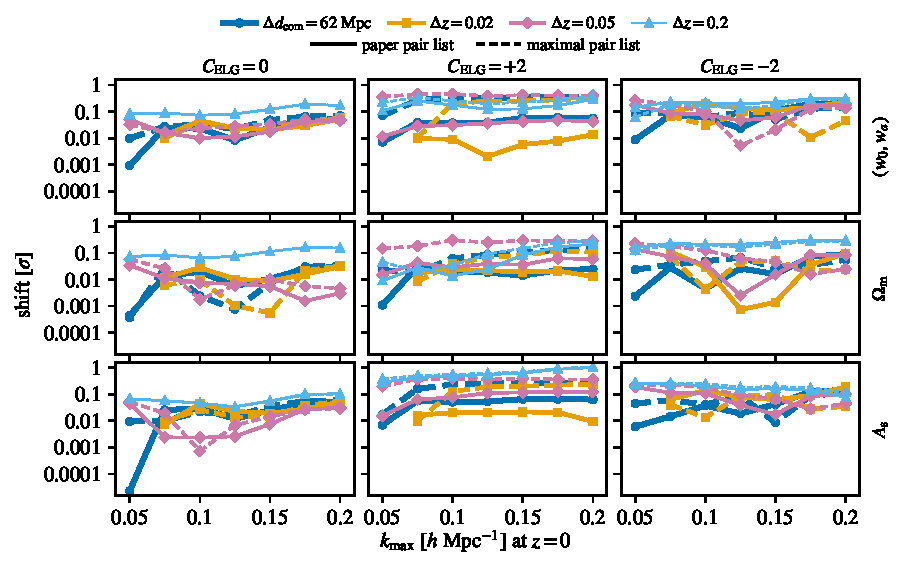
\includegraphics[width=\linewidth]{plots/mag_shift_kmax/mag_shift_kmax.pdf}
  \caption{The shift test against the scale cut: what-if MCMC-safety
    estimates of where the magnification-free fit lands if nature
    carries magnification at the stated coefficients.  Rows: the
    $(w_0, w_a)$ shift in units of its error ellipse, and the
    absolute shifts of $\Omega_m$ and $A_s$ in units of their
    marginalized errors.  Columns: $C_{\rm ELG} = 0$, $+2$ and $-2$,
    with BGS $C = 2$ and LRG $C = 3$ throughout.  The four layouts
    are distinguished by colour, line width and marker; solid lines
    are the paper pair lists, dashed lines the maximal (pairmax)
    lists.  Every nuisance is free; the frozen (cosmology-only)
    values are in the text and the run records.  The shared vertical
    axis is logarithmic, the quoted $\kmax$ is the $z = 0$ value of
    the per-bin cut at $\kmax/D(\bar z_i)$, and no threshold line is
    drawn.}
  \label{fig:shift}
\end{figure}

\paragraph{What the numbers say.}
\emph{At the measured coefficients} ($C_{\rm ELG} = 0$), leaving
magnification out moves the thin-layout fits by at most about $0.07$
of the error, on both pair lists; adding the pairmax pairs barely
changes the shifts, because magnification across two to four
thin-bin widths is still small (Section~\ref{sec:handworked}).
\emph{The unmeasured ELG count slope dominates.}  At
$C_{\rm ELG} = -2$ the paper lists reach $0.2$--$0.3$; at
$C_{\rm ELG} = +2$ the pairmax lists reach $0.30$--$0.46$ against at
most $0.06$ on the thin paper lists.  In that corner the free
nuisances make the shift \emph{larger}, not smaller (on
$\Delta z = 0.05$ pairmax: free $0.46$, frozen $0.20$): the added
pairs' magnification reads as a change of the per-group linear-bias
level and slope, exactly the freedom whose extra constraint produces
the pairmax FoM gain (\texttt{notes/cross\us correlations}).  The
gain and the magnification sensitivity are two faces of the same
channel.  \emph{At the fiducial coefficients the nuisance freedom
absorbs most of the signal}: holding the nuisances fixed raises the
$(w_0, w_a)$ shift by a factor $1.5$ to $13$ cut by cut (more where
the free shift nearly vanishes); at the maxima over cuts the factor
is $1.7$ to $3.5$ on the thin layouts and $1.6$ on
$\Delta z = 0.2$.
\emph{$\Delta z = 0.2$ is different in kind}: its cross spectra are
magnification dominated (Section~\ref{sec:estimate}), it moves
$0.19$ even at the fiducial coefficients, and its $A_s$ shifts by
about $1\sigma$ at $C_{\rm ELG} = +2$.  Its FoM is the smallest of
the four layouts, so this matters for the wide-bin comparison rather
than for the headline forecasts.

\section{Magnification in the model}
\label{sec:inmodel}

If the shift-test numbers are judged too large to leave the term out
-- or if the pair list is ever extended toward genuinely far pairs --
the coefficients move into the model.  The method is fixed by the
structure of the signal; only the results wait.

\paragraph{Exact template columns.}
The data vector is linear in each $C_i$ through the terms that cross
density with magnification, and quadratic through the magnification
auto terms; nothing else depends on the coefficients.  Each coefficient's derivative column is therefore
an exact template -- a handful of evaluations per group isolates the
linear and quadratic pieces algebraically, with no stencil noise --
exactly as the project already treats the stochastic amplitudes.
With one coefficient per sample group there are six new columns.

\paragraph{The cosmology columns change.}
The magnification terms carry $\Omega_m$, the growth factor and the
distances, so every cosmology derivative must be recomputed with the
coefficients on: the cached magnification-free derivative bases serve
the shift test, not the extended forecast.  The runtime cost (the
magnification kernels widen every lens bin's quadrature support to
the full foreground) is measured before this step is scheduled.

\paragraph{Coefficient treatments.}
Three treatments, in increasing order of caution: fixed at the
measured values (DES~Y3's baseline, justified there by the
fixed-versus-Gaussian difference being $0.06$--$0.19\sigma$ in $S_8$
\cite{ElvinPoole2022}); Gaussian priors at the measurement widths;
free.  With far pairs in the data vector the free treatment becomes
self-calibrating -- the cross spectra measure the coefficients
\cite{ElvinPoole2022, Sailer2025, MontanariDurrer2015} -- and
magnification turns from a nuisance into a signal.

\pending{T3 results: ${\rm FoM}(w_0, w_a)$ and ${\rm FoM}(\Omega_m,
10^9 A_s)$ against $\kmax$ with the coefficients off / fixed /
Gaussian / free, paper and pairmax lists (figure
\texttt{mag\us fom\us cost}); and, if the far-pair extension T4 runs,
$\sigma(C_g)$ against the pair reach (figure
\texttt{mag\us selfcal}).  Before the exact-template derivative
columns are built, the autos' $5\times10^{-3}$ polynomial-response
residual (Section~\ref{sec:guard}) must be traced.}

\appendix

\section{Open issues}
\label{sec:open}

\begin{itemize}
\item \textbf{The ELG count slope is unmeasured.}  Table~\ref{tab:coeff}
  brackets $C_{\rm ELG}$ in $[-2, +2]$; the finite-difference
  measurement on the DESI ELG target selection (with the
  fibre-magnitude response, Section~\ref{sec:measure}) replaces the
  bracket when it runs.
\item \textbf{The ``Limber-safe'' hand-off is untested for thin
  pairs.}  The FKEM magnification row is exact at linear level; its
  nonlinear correction rides Limber on the assertion that the broad
  kernel is safe (\texttt{cosmo2D.c:76--78}).  One brute-force
  spherical-Bessel check on a thin pair settles it
  (Section~\ref{sec:guard}, the one validation not yet run).
\item \textbf{The autos' polynomial-response residual.}  The
  four-point linearity identity closes to $10^{-5}$ of $\delta d$ on
  the cross pairs but only to $5\times10^{-3}$ on the autos
  (Section~\ref{sec:guard}); the residual sits in the auto
  non-Limber rows and must be traced before the exact-template
  coefficient derivatives of Section~\ref{sec:inmodel} are built.
\item \textbf{The scale cuts were built without magnification.}
  On $\Delta z = 0.2$ most of the pairmax magnification signal falls
  outside the ultraviolet-fraction cuts
  (Section~\ref{sec:estimate}); a cut rebuilt on the model with
  magnification would keep different bands.
\item \textbf{Doppler terms at low redshift.}  The leading omitted
  count term; the estimate for the lowest-$z$ BGS adjacent pairs is
  pending (Section~\ref{sec:omitted}).
\item \textbf{Far pairs.}  Beyond the pairmax lists magnification is
  both mandatory in the model and a measurable signal; whether the
  data vector is ever extended that far is a separate decision, with
  the self-calibration forecast (T4) as its input.
\end{itemize}

\begin{thebibliography}{99}

\bibitem{ChallinorLewis2011}
A.~Challinor and A.~Lewis,
``The linear power spectrum of observed source number counts'',
Phys.\ Rev.\ D 84 (2011) 043516, arXiv:1105.5292.

\bibitem{BonvinDurrer2011}
C.~Bonvin and R.~Durrer,
``What galaxy surveys really measure'',
Phys.\ Rev.\ D 84 (2011) 063505, arXiv:1105.5280.

\bibitem{Yoo2009}
J.~Yoo, A.~L. Fitzpatrick and M.~Zaldarriaga,
``A new perspective on galaxy clustering as a cosmological probe:
general relativistic effects'',
Phys.\ Rev.\ D 80 (2009) 083514, arXiv:0907.0707.

\bibitem{KrauseY3}
E.~Krause, X.~Fang, S.~Pandey et al.\ (DES),
``Dark Energy Survey Year 3 results: multi-probe modeling strategy
and validation'',
2021, arXiv:2105.13548.

\bibitem{ElvinPoole2022}
J.~Elvin-Poole, N.~MacCrann, S.~Everett et al.\ (DES),
``Dark Energy Survey Year 3 results: magnification modeling and
impact on cosmological constraints from galaxy clustering and
galaxy-galaxy lensing'',
2022, arXiv:2209.09782.

\bibitem{Fang2020}
X.~Fang, E.~Krause, T.~Eifler and N.~MacCrann,
``Beyond Limber: efficient computation of angular power spectra for
galaxy clustering and weak lensing'',
2020, arXiv:1911.11947.

\bibitem{JelicCizmek2021}
G.~Jelic-Cizmek, F.~Lepori, C.~Bonvin and R.~Durrer,
``On the importance of lensing for galaxy clustering in photometric
and spectroscopic surveys'',
2021, arXiv:2004.12981.

\bibitem{EuclidSpectroMag}
Euclid Collaboration: G.~Jelic-Cizmek, F.~Sorrenti, F.~Lepori et al.,
``Euclid preparation: impact of magnification on spectroscopic
galaxy clustering'',
2023, arXiv:2311.03168.

\bibitem{LeporiEuclid}
Euclid Collaboration: F.~Lepori, I.~Tutusaus, C.~Viglione et al.,
``Euclid preparation: XIX. Impact of magnification on photometric
galaxy clustering'',
2022, arXiv:2110.05435.

\bibitem{MontanariDurrer2015}
F.~Montanari and R.~Durrer,
``Measuring the lensing potential with tomographic galaxy number
counts'',
2015, arXiv:1506.01369.

\bibitem{Cardona2016}
W.~Cardona, R.~Durrer, M.~Kunz and F.~Montanari,
``Lensing convergence and the neutrino mass scale in galaxy redshift
surveys'',
2016, arXiv:1603.06481.

\bibitem{Thiele2020}
L.~Thiele, C.~A.~J. Duncan and D.~Alonso,
``Disentangling magnification in combined shear-clustering
analyses'',
2020, arXiv:1907.13205.

\bibitem{Pandey2023}
S.~Pandey, C.~S\'anchez and B.~Jain (LSST DESC),
``Cosmology with imaging galaxy surveys: the impact of evolving
galaxy bias and magnification'',
2023, arXiv:2310.01315.

\bibitem{Wenzl2023}
L.~Wenzl, S.-F. Chen and R.~Bean,
``Magnification bias estimators for realistic surveys: an application
to the BOSS survey'',
2023, arXiv:2308.05892.

\bibitem{Zhou2023}
R.~Zhou, S.~Ferraro, M.~White et al.,
``DESI luminous red galaxy samples for cross-correlations'',
2023, arXiv:2309.06443.

\bibitem{KitanidisWhite2020}
E.~Kitanidis and M.~White,
``Cross-correlation of Planck CMB lensing with DESI-like LRGs'',
2020, arXiv:2010.04698.

\bibitem{Sailer2025}
N.~Sailer, J.~DeRose, S.~Ferraro et al.,
``Evolution of structure growth during dark energy domination:
insights from the cross-correlation of DESI galaxies with CMB
lensing and galaxy magnification'',
2025, arXiv:2503.24385.

\bibitem{Saraivanov2026}
E.~Saraivanov, H.~Rubira, V.~Miranda and T.~Eifler,
``Towards the Two-Loop EFTofLSS in Galaxy Lensing Surveys'',
2026, arXiv:2603.13031.

\end{thebibliography}

\end{document}
